\tikzset
{
    vnodeStyle/.style =
    {
        % -- shape properties --
        circle,                                 % shape
        minimum size    = 7mm,                %
        scale           = 1.0,                  % scaling factor
        thick,                                  % thickness of the border
        %
        % -- colours properties --
        % filling: [ trasparent | monocolored | shaded]; decomment what you prefer
%       %                                       % transparent (all commented)
        fill            = yellow!10,             % monocolored
        text            = black,                % colour of the fonts
        draw            = black,                % colour of the border
        %
        % -- fonts --
        font            = \scriptsize,              % shape of the font (or dimension, like \tiny)
%       text centered,                          % text alignment [text centered | text badly centered | text justified | text ragged | text badly ragged]
        inner xsep      = 0mm,                  % minimum distance between text and borders along x dimension
        inner ysep      = 0mm,                  % minimum distance between text and borders along y dimension
        text height     = 0.2cm,
        text depth      = 0.12cm,
    }
}

%\begin{center}
\tikzstyle{styB}=[circle,
  ball color=blue,
  inner sep=0pt,
  minimum size=10pt]
\tikzstyle{styKB}=[circle,
  ball color=blue!10!white,
  inner sep=0pt,
  minimum size=10pt]
\tikzstyle{styCd}=[rectangle, draw=blue!50,
  top color=blue!40!white, bottom color=blue!10,
  inner sep=0pt,
  minimum size=10pt]
\tikzstyle{styCu}=[rectangle, draw=blue,
  top color=blue, bottom color=blue!40,
  inner sep=0pt,
  minimum size=10pt]

\pgfdeclarelayer{background}
%
\pgfdeclarelayer{foreground}
%
\pgfdeclarelayer{m-f}
%
\pgfdeclarelayer{main}
%
\pgfsetlayers{background,main,m-f,foreground}

\begin{tikzpicture}[scale=2.0]
% \draw[step=5mm,color=gray!40!white, thin] (0,0) grid (12,5);

\colorlet{uecolr}{black} \colorlet{decolr}{black!40}

\def\strt  {-40mm}
\def\shf   {10mm}
\def\ang   {55}
\def\dist  {4mm}
\def\cvd   {18mm}

\def\n     {6}
\def\s     {7}

\begin{scope}[xshift=-7cm, yshift=-1.2cm]

\only<1>
{
%\node (cc) at (12mm,5mm) {Product Code\vphantom{y}};

\foreach \rr in {0,1,...,\n}
 \foreach \cc in {0,1,...,\n}
  \node[vnodeStyle] (p\rr\cc) at (\rr*4mm,-\cc*4mm) {$X_{\cc,\rr}$};

 \node [rectangle,rounded corners=2mm,minimum width=7mm,minimum height=55mm,draw=red,thick] (circ1) at (4mm,-12mm) {};
 \node [rectangle,rounded corners=2mm,minimum width=55mm,minimum height=7mm,draw=red,thick] (circ2) at (12mm,-4mm) {};
}

\only<2>
{
%\node (cc) at (12mm,5mm) {Product Code\vphantom{y}};

\foreach \rr in {0,1,...,\n}
 \foreach \cc in {0,1,...,\n}
  \node[vnodeStyle] (p\rr\cc) at (\rr*4mm,-\cc*4mm) {$X_{\cc,\rr}$};

 \node [rectangle,rounded corners=2mm,minimum width=39mm,minimum height=39mm,draw=black,thick] (circ1) at (8mm,-8mm) {};
 \node [rectangle,rounded corners=2mm,minimum width=14mm,minimum height=55mm,draw=blue,thick] (circ1) at (22mm,-12mm) {};
 \node [rectangle,rounded corners=2mm,minimum width=55mm,minimum height=14mm,draw=red,thick] (circ2) at (12mm,-22mm) {};
}

%\only<2>
%{
%\node (cc) at (12mm,5mm) {Symmetric Subcode};
%
%\foreach \cc in {0,1,...,\n}
%  \foreach \rr in {\cc,...,\n}
%    \node[vnodeStyle] (p\rr\cc) at (\rr*4mm,-\cc*4mm) {$X_{\cc,\rr}$};
%
%\pgfmathtruncatemacro{\nnn}{\n-1}
%\foreach \rr in {0,1,...,\nnn} {
%  \pgfmathtruncatemacro{\rrr}{\rr+1}
%  \foreach \cc in {\rrr,...,\n}
%    \node[vnodeStyle] (p\rr\cc) at (\rr*4mm,-\cc*4mm) {$X_{\color{red}{\rr,\cc}}$};
%}
%
% \node [rectangle,rounded corners=2mm,minimum width=7mm,minimum height=55mm,draw=red,thick] (circ1) at (4mm,-12mm) {};
% \node [rectangle,rounded corners=2mm,minimum width=55mm,minimum height=7mm,draw=red,thick] (circ2) at (12mm,-4mm) {};
%}

%\only<3>
%{
%\node (cc) at (12mm,5mm) {Punctured Symmetric Subcode};
%
%\foreach \cc in {0,1,...,\n}
%  \foreach \rr in {\cc,...,\n}
%    \node[vnodeStyle] (p\rr\cc) at (\rr*4mm,-\cc*4mm) {$X_{\cc,\rr}$};
%
% \node [rectangle,rounded corners=2mm,minimum width=7mm,minimum height=15mm,draw=red,thick] (circ1) at (4mm,-2mm) {};
% \node [rectangle,rounded corners=2mm,minimum width=47mm,minimum height=7mm,draw=red,thick] (circ2) at (14mm,-4mm) {};
%}


%\foreach \rr in {0,1,...,\n}{
% \node [rectangle,rounded corners=1mm,minimum width=4mm,minimum height=\n*4mm+4mm,draw=red,thick] (circ1) at (1*4mm,3*4mm) {};
% \node [rectangle,rounded corners=1mm,minimum width=\n*4mm+4mm,minimum height=4mm,draw=maroon,thick] (circ2) at (3*4mm,1*4mm) {};
% \node (cc) at (12mm,29mm) {column codewords};
% \node [rotate=90](rc) at (-6mm,12mm) {row codewords};
% }
\end{scope}

\end{tikzpicture}
%\end{center}
